\documentclass{article}
\usepackage[margin=0.1in]{geometry}
\usepackage{url}
\usepackage{multicol}
\usepackage{amsmath}
\usepackage{esint}
\usepackage{amsfonts}
\usepackage{tikz}
\usetikzlibrary{decorations.pathmorphing}
\usepackage{amsmath,amssymb}

\usepackage{colortbl}
\usepackage{xcolor}
\usepackage{mathtools}
\usepackage{amsmath,amssymb}
\usepackage{enumitem}

\newcommand{\blank}[1]{\hspace*{#1}\linebreak[0]}

\tikzstyle{mybox} = [draw=black, fill=white, very thick,
    rectangle, rounded corners, inner sep=10pt, inner ysep=10pt]
\tikzstyle{fancytitle} =[fill=black, text=white, font=\bfseries]

\begin{document}
\begin{center}{\huge{\textbf{CS 480 Cheat Sheet}}}
\end{center}

\begin{multicols*}{2}
%------------ Perceptron ---------------------
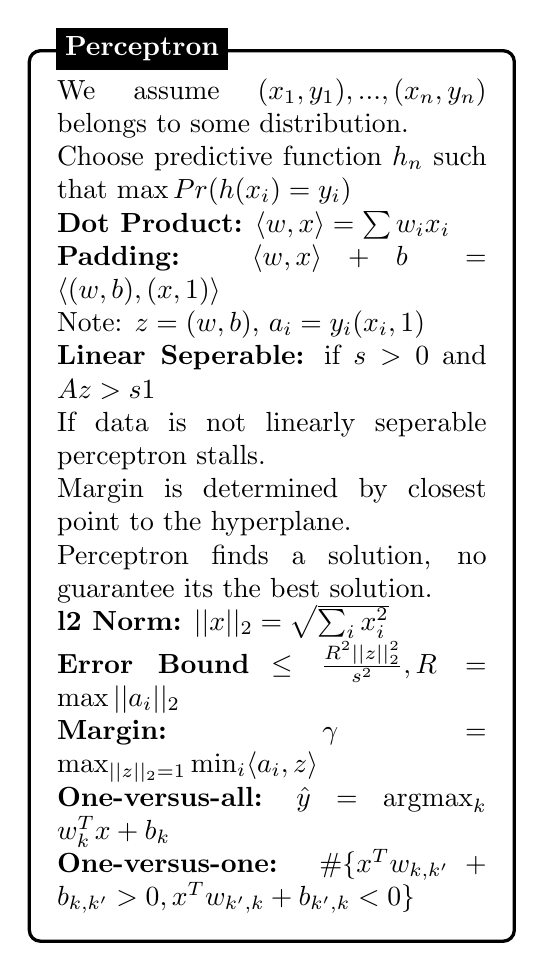
\begin{tikzpicture}
\node [mybox] (box){%
    \begin{minipage}{0.45\textwidth}
    We assume $(x_1,y_1),...,(x_n,y_n)$ belongs to some distribution.\\
    Choose predictive function  $h_n$ such that $\max Pr(h(x_i) = y_i)$ \\
    \textbf{Dot Product:} $ \langle w, x  \rangle = \sum w_ix_i $\\
    \textbf{Padding:} $\langle w, x  \rangle + b = \langle (w, b), (x, 1) \rangle$ \\
    Note: $z = (w,b)$, $a_i = y_i(x_i,1)$\\
    \textbf{Linear Seperable:} if $s>0$ and $Az > s1$ \\
If data is not linearly seperable perceptron stalls. \\
Margin is determined by closest point to the hyperplane. \\
Perceptron finds a solution, no guarantee its the best solution. \\
    \textbf{l2 Norm:} $||x||_2 = \sqrt{\sum_ix_i^2}$ \\
    \textbf{Error Bound} $\leq \frac{R^2||z||^2_2}{s^2}, R = \max||a_i||_2$  \\
    \textbf{Margin:} $\gamma = \max_{||z||_2 = 1} \min_i \langle a_i, z \rangle$ \\
    \textbf{One-versus-all:}  $\hat{y} = \text{argmax}_k$ $w_k^Tx + b_k $ \\
    \textbf{One-versus-one:} $\# \{ x^Tw_{k,k'} + b_{k,k'} > 0, x^Tw_{k',k} + b_{k',k} < 0 \}$
    \end{minipage}
};
\node[fancytitle, right=10pt] at (box.north west) {Perceptron};
\end{tikzpicture}

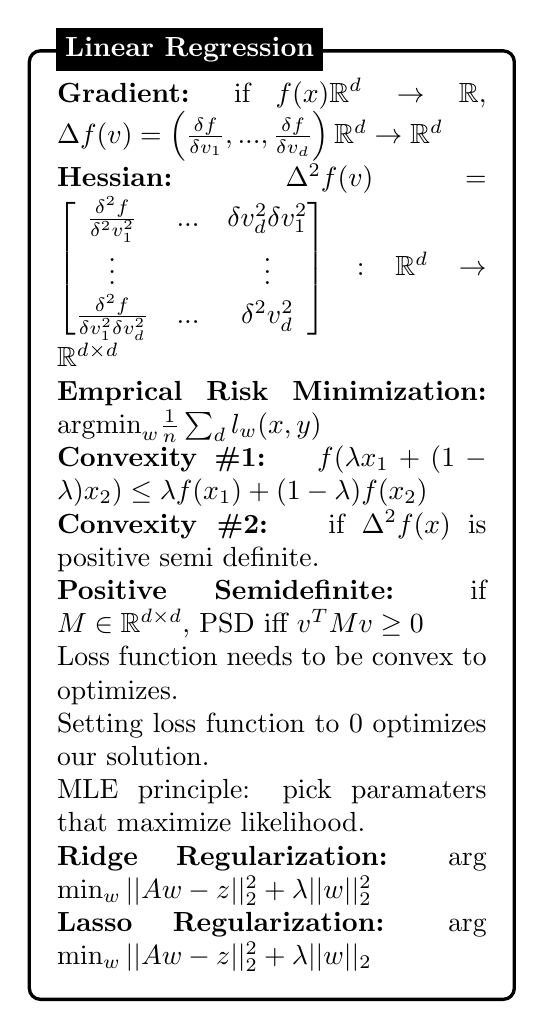
\begin{tikzpicture}
\node [mybox] (box){%
    \begin{minipage}{0.45\textwidth}
	\textbf{Gradient:} if $f(x) \mathbb{R}^d \rightarrow \mathbb{R}$, $\Delta f(v) = \left( \frac{\delta f}{\delta v_1}, ..., \frac{\delta f}{\delta v_d}  \right) \mathbb{R}^d \rightarrow \mathbb{R}^d$ \\
	\textbf{Hessian:} $\Delta^2 f(v) = \begin{bmatrix}
\frac{\delta^2f}{\delta^2 v_1^2} & ... & \delta v_d^2\delta v_1^2 \\
\vdots &  & \vdots \\
\frac{\delta^2f}{\delta v_1^2\delta v_d^2} & ... & \delta^2 v_d^2
\end{bmatrix}: \mathbb{R}^d \rightarrow\mathbb{R}^{d\times d} $\\
\textbf{Emprical Risk Minimization:} $\text{argmin}_w \frac{1}{n}\sum_d l_w(x,y)$ \\
\textbf{Convexity \#1: } $f(\lambda x_1 + (1- \lambda)x_2) \leq \lambda f(x_1) + (1-\lambda)f(x_2)$ \\
\textbf{Convexity \#2: } if $\Delta^2f(x)$ is positive semi definite. \\
\textbf{Positive Semidefinite:} if $M \in \mathbb{R}^{d \times d}$, PSD iff $v^TMv \geq 0$\\
Loss function needs to be convex to optimizes.\\
Setting loss function to 0 optimizes our solution.\\
MLE principle: pick paramaters that maximize likelihood.\\
\textbf{Ridge Regularization:} arg $\min_w ||Aw-z||^2_2 + \lambda||w||^2_2
$\\
\textbf{Lasso Regularization:} arg $\min_w ||Aw-z||^2_2 + \lambda||w||_2
$    \end{minipage}
};
\node[fancytitle, right=10pt] at (box.north west) {Linear Regression};
\end{tikzpicture}

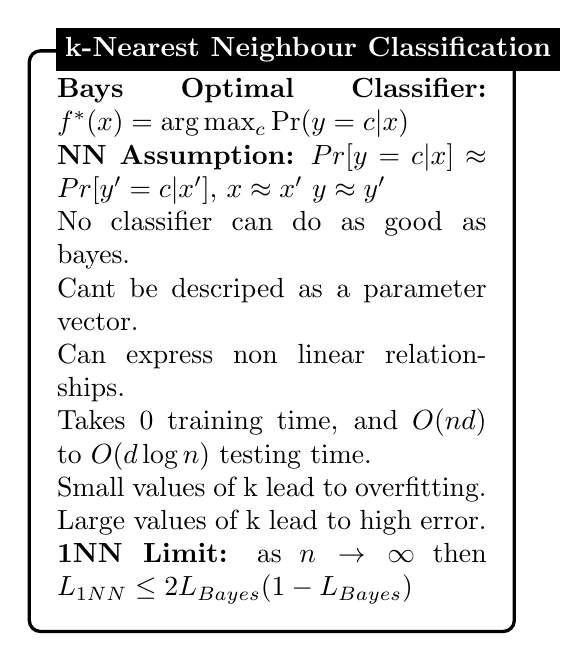
\begin{tikzpicture}
\node [mybox] (box){%
    \begin{minipage}{0.45\textwidth}
	\textbf{Bays Optimal Classifier:} $f^*(x) = \text{arg}\max_c\text{Pr}(y=c|x)$\\
	\textbf{NN Assumption:} $Pr[y=c|x] \approx Pr[y'=c|x']$, $x\approx x'$ $y \approx y'$\\
	No classifier can do as good as bayes.\\
	Cant be descriped as a parameter vector.\\
	Can express non linear relationships.\\
	Takes 0 training time, and $O(nd)$  to $O(d\log n)$ testing time.\\
	Small values of k lead to overfitting. \\
	Large values of k lead to high error. \\
	\textbf{1NN Limit:} as $n \rightarrow \infty$ then $L_{1NN} \leq 2L_{Bayes}(1 - L_{Bayes})$

    \end{minipage}
};
\node[fancytitle, right=10pt] at (box.north west) {k-Nearest Neighbour Classification};
\end{tikzpicture}

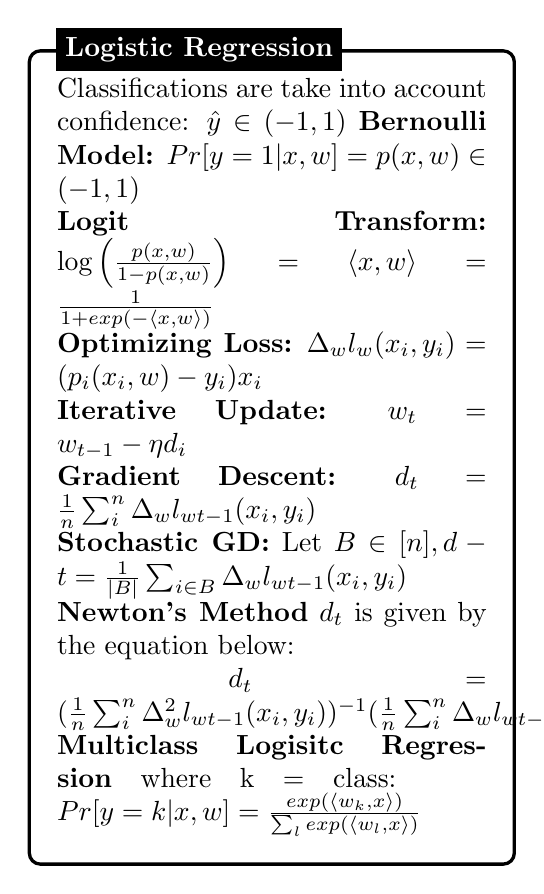
\begin{tikzpicture}
\node [mybox] (box){%
    \begin{minipage}{0.45\textwidth}
		Classifications are take into account confidence: $\hat{y} \in (-1,1)$
		\textbf{Bernoulli Model:} $Pr[y=1|x,w] = p(x,w) \in (-1,1) $ \\
		\textbf{Logit Transform:} $\log\left( \frac{p(x,w)}{1-p(x,w)}\right) = \langle x,w\rangle = \frac{1}{1+exp(-\langle x,w\rangle)}$\\
		\textbf{Optimizing Loss:} $\Delta_w l_w(x_i,y_i) = (p_i(x_i,w)-y_i)x_i$\\
		\textbf{Iterative Update:} $w_t = w_{t-1}-\eta d_i$ \\
		\textbf{Gradient Descent:} $d_t = \frac{1}{n}\sum_i^n\Delta_w l_{wt-1}(x_i,y_i)$ \\
		\textbf{Stochastic GD:} Let $B \in [n], d-t = \frac{1}{|B|}\sum_{i\in B}\Delta_w l_{wt-1}(x_i,y_i)$ \\
		\textbf{Newton's Method} $d_t$ is given by the equation below:\\
		\blank{0.5cm} $d_t = (\frac{1}{n}\sum_i^n\Delta^2_w l_{wt-1}(x_i,y_i))^{-1}(\frac{1}{n}\sum_i^n\Delta_w l_{wt-1}(x_i,y_i))$\\
		\textbf{Multiclass Logisitc Regression} where k = class:
		\blank{0.5cm} $Pr[y=k|x,w] = \frac{exp(\langle w_k,x \rangle)}{\sum_l exp(\langle w_l,x \rangle)} $
    \end{minipage}
};
\node[fancytitle, right=10pt] at (box.north west) {Logistic Regression};
\end{tikzpicture}
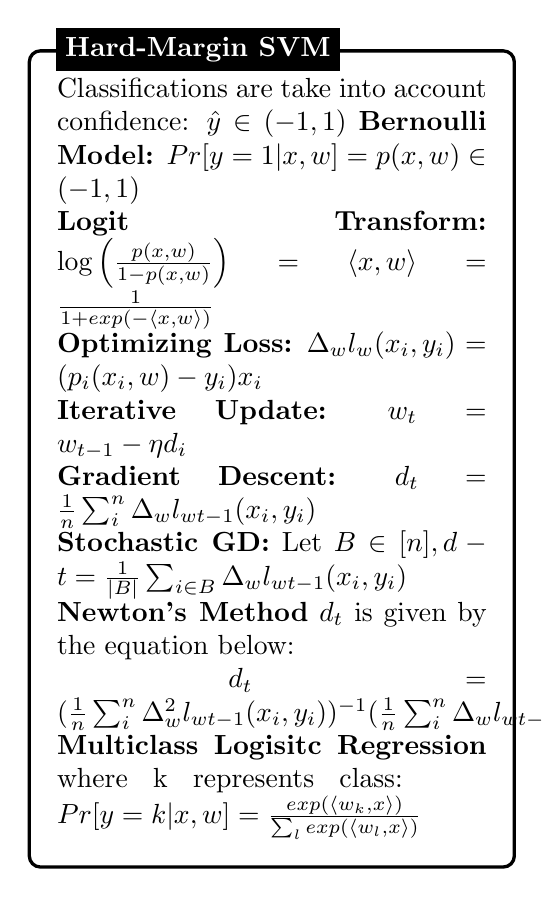
\begin{tikzpicture}
\node [mybox] (box){%
    \begin{minipage}{0.45\textwidth}
		Classifications are take into account confidence: $\hat{y} \in (-1,1)$
		\textbf{Bernoulli Model:} $Pr[y=1|x,w] = p(x,w) \in (-1,1) $ \\
		\textbf{Logit Transform:} $\log\left( \frac{p(x,w)}{1-p(x,w)}\right) = \langle x,w\rangle = \frac{1}{1+exp(-\langle x,w\rangle)}$\\
		\textbf{Optimizing Loss:} $\Delta_w l_w(x_i,y_i) = (p_i(x_i,w)-y_i)x_i$\\
		\textbf{Iterative Update:} $w_t = w_{t-1}-\eta d_i$ \\
		\textbf{Gradient Descent:} $d_t = \frac{1}{n}\sum_i^n\Delta_w l_{wt-1}(x_i,y_i)$ \\
		\textbf{Stochastic GD:} Let $B \in [n], d-t = \frac{1}{|B|}\sum_{i\in B}\Delta_w l_{wt-1}(x_i,y_i)$ \\
		\textbf{Newton's Method} $d_t$ is given by the equation below:\\
		\blank{0.5cm} $d_t = (\frac{1}{n}\sum_i^n\Delta^2_w l_{wt-1}(x_i,y_i))^{-1}(\frac{1}{n}\sum_i^n\Delta_w l_{wt-1}(x_i,y_i))$\\
		\textbf{Multiclass Logisitc Regression} where k represents  class:
		\blank{0.5cm} $Pr[y=k|x,w] = \frac{exp(\langle w_k,x \rangle)}{\sum_l exp(\langle w_l,x \rangle)} $
    \end{minipage}
};
\node[fancytitle, right=10pt] at (box.north west) {Hard-Margin SVM};
\end{tikzpicture}
\end{multicols*}

\end{document}